% Created 2018-01-19 Fr 12:26
% Intended LaTeX compiler: pdflatex
\documentclass{scrartcl}
\usepackage[utf8]{inputenc}
\usepackage[T1]{fontenc}
\usepackage{graphicx}
\usepackage{grffile}
\usepackage{longtable}
\usepackage{wrapfig}
\usepackage{rotating}
\usepackage[normalem]{ulem}
\usepackage{amsmath}
\usepackage{textcomp}
\usepackage{amssymb}
\usepackage{capt-of}
\usepackage{hyperref}
\usepackage{siunitx}
\usepackage{adjustbox}
\usepackage{colortbl}
\usepackage{subcaption}
\usepackage{natbib}
\newcommand{\whocares}{WHO$_2$CARES }
\author{Prudence Bateson, Prateek Dongre, Margarita Kaznacheeva,\\ Caterina Peris, Simon Pfreundschuh, Maxime Prignon,\\  Thomas Produit, Ahmet Mustafa Tepe, Samuel Weber}
\date{\today}
\title{WHO$_2$CARES - Mission Proposal}
\hypersetup{
 pdfauthor={Prudence Bateson, Prateek Dongre, Margarita Kaznacheeva,\\ Caterina Peris, Simon Pfreundschuh, Maxime Prignon,\\  Thomas Produit, Ahmet Mustafa Tepe, Samuel Weber},
 pdftitle={WHO$_2$CARES - Mission Proposal},
 pdfkeywords={},
 pdfsubject={},
 pdfcreator={Emacs 24.5.1 (Org mode 9.0.8)}, 
 pdflang={English}}
\begin{document}

\maketitle

\section{Background}
\label{sec:org1347442}

The \whocares satellite cluster will monitor the Earth’s surface and troposphere
at a higher spectral and temporal resolution of any satellite system of its
kind. Its primary foci are across various useful earth science observations:
clouds, aerosols, surface reflectance, and the oxygen A-band. Each of these
retrievals is discussed in more detail below. These measurements are
particularly valued for ongoing studies of anthropogenic climate change.

\subsection{Existing Technologies}
\label{sec:org43b3706}

Current state-of-the-art Earth Observing (EO) satellites
and sensors offer some view into cloud, aerosol, albedo, and land use. This is
done, in part, using the visible and near infrared (NIR) parts of the
electromagnetic spectrum. The \whocares satellite cluster will refine and
miniaturize these technologies, bringing them to the cutting edge of
nano-satellite design. \whocares will offer fast temporal resolution, regional
scale spatial resolution, and hyperspectral sensors to monitor fast-moving and
diverse environments on our Earth’s surface and in the troposphere. \whocares
also gives a completely new design facet of 3-dimensional data builds, with
satellite looking pairs in the cluster offering 3D geometric resolution of
surface features and cloud tops.

At first, it is pertinent to explore the existing state-of-the-art to discover
how the visible-NIR has been observed in the past and how we can effectively
build upon this great wealth of satellite EO data.

\subsubsection{Hyperion (earth Observing-1)}
\label{sec:org37e5de5}

Hyperion was a hyperspectral, high-resolution
imaging instrument aboard the experiment Earth Observing-1 (EO-1) satellite.
Originally launched in 2000, it was expected to have a lifetime of 1 year but it
far extended this, reaching a total life time of 17 years. EO-1 was deactivated
in 2017. It had 220 unique channels with a spectral bandwidth of just 10 nm,
across a spectral range of 0.4 – 2.5 µm. Despite a primary mission of validating
the instruments aboard, EO-1 provided some land imagery that was coupled with
LandSat 7 to validate quality. Another great achievement of Hyperion was a
ground resolution of 30m, allowing less-than regional scale observations to be
made. These highly advanced spectral and spatial resolutions came at the cost of
temporal resolution, with a total of 16 days return time \citep{principles}.

\subsubsection{MISR}
\label{sec:org8418862}

Multi-angle Imaging SpectroRadiometer (MISR) can distinguish the volume and
types of atmospheric aerosols particles, the types and height of clouds, and the
distribution of land surface cover \citep{diner}. MISR offers nine
viewing angles to resolve geometric variations across observed scenes. MISR also
operates in 4 different channels; red, green, blue, and near-infrared. MISR is a
specialist instrument for cloud top height and pressure retrievals, cloud
albedo, aerosol characterization and mapping, and land surface albedo and
classification. These technologies are now validated and can be adapted across
\whocares system. \whocares offers a higher spectral and temporal resolution
thus offering features like a more precise pressure-temperature profile and the
ability to model within the diurnal cycle.

\subsubsection{MODIS}
\label{sec:org3363f5b}

Moderate Resolution Imaging Spectroradiometer (MODIS) is an instrument
operating on the Terra and Aqua NASA spacecraft, first flown in 1999 and again
in 2002 \citep{modis}. It offers a view of the atmosphere, land, and
ocean measuring across the visible and infrared spectrum. Although not offering
the stereoscopic properties of MISR (above), it has a high spectral, spatial,
and temporal resolution. MODIS is key player in the current studies of global
cloud cover and cloud height. It also offers land use products such as
vegetation indices, burned area products, and ocean colour features. The ability
to not only provide moderate to high resolution products, but also offer so many
products to the end user, displays the power of MODIS. To provide a higher
temporal and spectral resolution, as well as a stereoscopic ability, across the
same suite of \whocares products to the scientific community would be
advantageous to all earth scientists with an interest in remote sensing.

\subsubsection{VIIRS}
\label{sec:orgdecaf60}

The Visible Infrared Imaging Radiometer Suite (VIIRS) is a sensor aboard
the Suomi NPP Weather satellite. On portion of its collected data are used as
environmental data records for the NOAA National Weather Service, whilst the
other portion stream through NASA and offer earth system data to the wider
community \citep{viirs}. The primary aim of VIIRS is to provide
complimentary cloud data to MODIS and other NASA instrumentation across sunlit
conditions in 12 bands, and an additional 9 infrared for surveying both night
and day clouds. It also offers smoke and fire detection and atmospheric aerosol
characterization and mapping \citep{viirs_book}. It offers slightly better
spatial and temporal resolution than MODIS, but at the cost of its spectral
resolution. \whocares will be building on this technology to provide
measurements on shorter timescales, although they \whocares products will not be
available in the mid- to long-wave infrared.

\subsubsection{TROPOMI}
\label{sec:orge34af6f}

The TROPOspheric Monitoring Instrument (TROPOMI) is primarily an atmospheric
chemistry instrument aboard the Sentinel-5p ESA satellite launched in 2017.
Alongside chemical species, it also monitors cloud fraction, albedo, and top
heights, and aerosol layer height \citep{tropomi}. TROPOMI data processing
can compute these using returns from the oxygen A-band, with a very high
spectral resolution. The <1nm spectral resolution comes at a loss of spatial
resolution, which is 3.5 – 7 km at nadir. The oxygen A-band will also be
measured in \whocares to give information on clouds and aerosols, offering a
much improved spatial and temporal resolution than TROPOMI.

\subsubsection{Flock (from Planet Lab Inc.)}
\label{sec:org7ced576}

The Flock is a nanosatellite cluster (and the only
nanosatellites to be discussed in this background) operated by private company
Planet Labs Inc. The Flock instruments are all loaded aboard a ‘Dove, a 3U
CubeSat, a nanosatellite standard of 10x10x30 cm. The satellite constellation
currently consists of \textasciitilde{}120 satellites, some of which were utilised as mechanical
and engineering tests, but with most capturing 4 band imagery of earth’s surface.
It is believed that a 3hr
temporal resolution can be achieved with a nanosatellite cluster of \textasciitilde{}92
CubeSats. Despite a significantly reducing spectral capture to a 3-band RGB
camera with one NIR component, the Doves can give a spatial resolution of 3 to 5
m. This resolution is useful for a community interested in small-scale local
changes, especially in land use or urbanisation.

However, \whocares wishes to give the scientific community a regional scale data
set to monitor changes on kilometre wide scales. By reducing the spatial
resolution, the spectral resolution can be improved with some hyperspectrality
brought in across the Vis-NIR wavelengths of interest. The high quality temporal
resolution that can only be given by such a dense network of nanosatellites is
of particular important when considering the state-of-art contribution offered
by Planet Lab Inc.’s designs.


\begin{table}[htbp]
\centering
\caption{Summary of relevant satellite missions}
\resizebox{\textwidth}{!}{%
\begin{tabular}{|p{6.5em}p{6.5em}cp{9em}p{11.145em}c|}
\hline
\rowcolor[rgb]{ 1.0,  1.0,  1.0} \textcolor[rgb]{ .0,  .0,  .0}{\textbf{Satellite/ Instrument}} & \textcolor[rgb]{ .0,  .0,  .0}{\textbf{Temporal Resolution}} & \multicolumn{1}{p{6.5em}}{\textcolor[rgb]{ .0,  .0,  .0}{\textbf{Spatial Resolution (km)}}} & \textcolor[rgb]{ .0,  .0,  .0}{\textbf{Spectral Range (µm)}} & \textcolor[rgb]{ 0.0,  .0,  .0}{\textbf{Spectral Bands or Hyperspectral Resolution}} & \multicolumn{1}{p{6.5em}|}{\textcolor[rgb]{ .0,  .0,  .0}{\textbf{Currently Active?}}} \\
\hline
\midrule
\textbf{Hyperion} & 16 days & 0.3   & 0.4 – 2.5 & Hyperspectral\newline{}10 nm & \multicolumn{1}{p{6.5em}|}{No} \\
\midrule
\textbf{MISR} & 9 days & \multicolumn{1}{p{6.5em}}{0.28 - 1} & 0.45 – 0.87 & 21.9 – 41.9 nm & \multicolumn{1}{p{6.5em}|}{Yes} \\
\midrule
\textbf{MODIS} & 1 – 2 days & \multicolumn{1}{p{6.5em}}{0.25 - 1} & 0.4 – 14.4 & 36 spectral bands & \multicolumn{1}{p{6.5em}|}{Yes} \\
\midrule
\textbf{VIIRS} & 1 day & \multicolumn{1}{p{6.5em}}{0.38 – 0.75} & 0.41 – 12.5 & 21 spectral bands & \multicolumn{1}{p{6.5em}|}{Yes} \\
\midrule
\textbf{TROPOMI} & 1 day & \multicolumn{1}{p{6.5em}}{3.5 - 7} & 0.27 – 0.78 with an extra 2.3-2.39 in IR & 0.25 – 0.54 nm & \multicolumn{1}{p{6.5em}|}{Yes\newline{}(fully online later 2018)} \\
\midrule
\textbf{Planet Labs} & 3 hrs & \multicolumn{1}{p{6.5em}}{0.03 – 0.05} & 0.45 – 0.86 & Up to 4 spectral bands & \multicolumn{1}{p{6.5em}|}{In Progress} \\
\midrule
\textbf{\whocares} & 3 hrs & 1     & 0.4 – 2 & Hyperspectral\newline{}2 nm - 10 nm &  \\
\hline
\bottomrule
\end{tabular}}%
\label{tab:addlabel}%
\end{table}

\subsection{Cloud Observations}
\label{sec:org850e761}


Accurate information on cloud properties, types, and their spatial and temporal
variation along the atmosphere is crucial for climate studies and models. Cloud
representations vary among global climate models, and small changes in cloud
cover have a large impact on the climate. Differences in planetary boundary
layer cloud modeling schemes can lead to large differences in derived values of
climate sensitivity. A model that decreases boundary layer clouds in response to
global warming has a climate sensitivity twice that of a model that does not
include this feedback.

Also, not all clouds are the same, different types of clouds affect the Earth’s
climate differently. Some types of clouds help to warm the Earth; others help
to cool it. The radiative effects of clouds depend strongly on cloud properties
such as thermodynamic phase, optical thickness and droplet effective radius.
The IPCC reported in 2007 that it projects the Earth’s average temperature to
be about 1.8 to 4 degrees Celsius higher by the end of the century than it was
in 1990 – a rapid rate of increase compared to observed rates of increase in
the Earth’s recent history.

Scientists could probably narrow down the Earth’s projected temperature range
 further if they better understood the relationships between clouds and climate
 as well as other factors, such as the amount of greenhouse gases that will be
 pumped into the atmosphere by 2100. Most scientists doubt that the net cooling
 effect of clouds will ever be large enough to completely offset ongoing warming.
 However, many scientists \citep{marshak} say that if warming were to increase the number
 of kind of cooling clouds or decrease the presence of warming clouds, the current net
cooling effect of clouds on the Earth’s climate would probably increase, and
thereby moderate, or offset, ongoing warming, and the Earth’s-end-of-the-century
temperature may be pulled down toward the lower end of its predicted range.

On the other hand, the opposite effect could happen and the upper end of the
predicted range is also possible and the increasing of the warming cycle would
be perpetuated.

The reason why clouds impact climate differently resides in their heights and
thickness. On the one hand, stratus clouds hang low in the sky – usually within
two kilometers of the Earth’s surface—and resemble a gray blanket covering
thousands of kilometers of sky. Because these clouds block sunlight from reaching
the Earth, they act like a sun-screen or shady umbrella that helps cool the Earth.
Therefore, they have a net cooling effect that helps offset warming.

Secondly, cirrus clouds are wispy and feathery, and positioned up to 20 kilometers
above the Earth’s surface. Cirrus clouds let much sunlight pass through them and
may also trap the Earth’s heat, just as greenhouse gases do. Therefore, they have
 a net warming effect that helps magnify warming.

Finally, Cumulus clouds, they extend vertically high in the sky. They have
sharply defined edges, may form alone, in lines or in clusters. Cumulus clouds
can block sunlight, but also trap the Earth’s heat. Their net effect on warming
depends on their heights and thicknesses.

Also, global warming is expected to change the distribution and type of clouds.
It is found that clouds are moving away from the equator as temperatures rise.
Subtropical dry zones have also been expanding. Observed and simulated cloud
change patterns are consistent with poleward retreat of mid-latitude storm
 tracks, expansion of subtropical dry zones, and increasing height of the
 highest cloud tops at all latitudes \citep{clouds_high}. These results indicate that the
 cloud changes most consistently predicted by global climate models are currently occurring in
 nature. Clouds heights do, however, vary considerably from year to year
 in connection with weather and
climate phenomena. La Niña and El Niño events have the strongest effect, with
the 2008 La Niña lowering global clouds on average by 40 meters and El Niño
events pushing the upward \citep{lelli}. Beyond that, the researchers found differences
in Southern Hemisphere and Northern Hemisphere cloud behavior and regional
correlations that warrant further investigation. With cloud heights naturally
varying so much, it is thought \citep{clouds_soon} that it could take at least 15 years of data
to spot any possible global effects of climate change. “All we can say at the
moment is that the global trends in cloud heights, if they are there, are being
swamped by El Niño – La Niña fluctuations”, “It will take a lot longer till we
can tease out these long-term trends.”. In terms of clouds, many efforts have
been dedicated to the retrieval of their properties and distribution along the
atmosphere. Passive satellite imagers are the most widely used instruments for
cloud retrievals as they provide long-term, global coverage at acceptable cost
for the user. The Advanced Very High Resolution Radiometer (AVHRR), on board the
NOAA satellites since the end of the 1970s, has been a significant contributor
to many global cloud climatologies. AVHRR with its four to six spectral channels
allows the retrieval of key cloud properties by abutting pixels that assemble a
seamless image. The heirs of the AVHRR were launched in several NASA/ESA
research missions, on board satellites such as Terra, Aqua, the European Remote
Sensing Satellite (ERS-1/2) and the Environmental Satellite (Envisat). Those are
the Moderate Resolution imaging Spectroradiometer (MODIS), the Along-Track
Scanning Radiometers (ATSR-1/2) and the Advanced Along-Track Scanning Radiometer
(AATSR), which provide an increased number of spectral channels as well as
higher spatial resolution (≤ 1 km footprint size) than AVHRR. The MODIS and
ATSR/AATSR sensors include the spectral channels of AVHRR but have additional
ones in the visible, near-infrared and, in the case of MODIS, also in the
thermal infrared. In addition, they have an increased spatial resolution as well
as contribution to increasing the observation frequency. The datasets derived
from these measurement retrievals are useful for climate studies and cover more
than one decade. ATSR provides its Global Retrieval of ATSR Cloud Parameters and
Evaluation (GRAPE; Sayer et al., 2011) for ATSR/AATSR, MODIS (NASA) its
Collection 5 (Platnick et al., 2015, 2017; Marchant et al., 2016). These cloud
properties datasets have now reached quality levels that facilitate qualitative
and quantitative assessments of clouds in the Earth’s climate system, even
availability to understand cloud processes and the evaluation of atmospheric
models. Till now, with visible and Near Infrarred bands cloud products such
Cloud Optical Thickness, Effective Radius, Liquid Water Content and Cloud Albedo
can be derived. There also have been some efforts devoted to obtain cloud
heights and cloud thickness through the analysis of the O2-A-Band changes by
means of sensors like SCIAMACHY/GOME/GOME-2. Given the high degree of
measurement accuracy afforded by current instruments, the reliability of derived
atmospheric products no longer depends as heavily on instrument calibration and
noise but more so on the choice of spectral bands, the forward model, and the
method of inversion. In addition there is still potential to improve the current
datasets. \whocares mission will offer a hyperspectrality, temporal resolution
and 3-Dimensional analysis of clouds that has not ever seen before. With its
higher spatial and temporal resolution products such as cloud optical thickness
can gain accuracy, and coupled with cloud heights retrieval through hyper
spectral analysis may help to derive new and improved cloud types products. This
could lead to finally determine the current trend of cloud heights and movement
due to global warming and climate change.


\subsection{Surface Observations}
\label{sec:org147f3dd}


MODIS has brought unprecedented data to scientists making
high quality, global datasets available to land, ocean and cryosphere
applications. \whocares aims to continue this legacy by observing the earth
in the visible and near infrared region in which the MODIS land and ocean
channels are located. Instead of 20 channels in this region, however,
\whocares will provide hyperspectral information with more than 100 channels.
This will open the door to a range of novel science applications, building upon
and extending the MODIS range of surface products.

\subsubsection{Land}
\label{sec:org188f852}

Synoptic and repetitive observations of vegetation cover and land use are
of great importance for the modeling and prediction of climate change as
well as the planning of urban and industrial development.

\begin{enumerate}
\item Vegetation
\label{sec:org772825a}

Besides regulating the regional carbon and hydrologic cycle, vegetation cover
has an important impact on atmsopheric composition and climate feedbacks. The
study of these processes require fine scale characterization of the
ecosystems involved. By providing high spectral resolution at moderate spatial
resolution, \whocares aims to close an important gap in the global monitoring
system of vegetation. Numerous studies have highlighted the potential of and
need for spaceborne hyperspectral observations. An example is the work by
\citet{haboudane} who developed robust, hyperspectral vegetation indices and
showed that they outperform the normalized difference vegetation index in the
prediction of green leaf area index (LAI). Furthermore, airborne hyperspectral
observations are commonly used for vegetation type classification. Relevant
applications of such informations can be found in the works of \citet{he}
who study the expansion of evergreens in the Siberian forest or \citet{winkler} 
who identify droughts affecting the agriculture in Africa.

\item Landuse and Disaster Response
\label{sec:org2a8ca68}

The revisiting inverval of three hours that will be achieved by \whocares
will further increase the frequency at which a given location is observed.
Clearly, the additional spectral information content of \whocares data will
allow a more detailed mapping of land use and land cover. Moreover, the
improved spatial resolution will be of great value for disaster response. As
an example, data from the MODIS instruments has been used to coordinate the
response in the wake of superstorm sandy. The biggest challenge with MODIS
data is cloud cover that obstructs the view on affected areas. Since
\whocares will see the same location twice as often as MODIS does, this will
greatly improve the probability to obtain useful live data for disaster
response.
\end{enumerate}

\subsubsection{Cryosphere}
\label{sec:orgf2dd4f7}

Observation in the visible and near infrared are commonly used to study regional and
global snow and ice cover. Applications are spatiotemporal snow cover variability
\citep{dariane, zhuo} and their impact on regional climate and hydrology. Also for 
observations of the cryosphere, the additional spectral information provided by
\whocares will help to improve our understanding and modeling of relevant processes.
Dozier and Painter show that hyperspectral observations of snow cover can be used
to determine both snow cover and snow albedo, which are important inputs for
cryosphere models.

\subsubsection{Ocean}
\label{sec:orgde76ad3}

With regards to the ocean, the additional spectral information delivered by \whocares
will allow to further extend on the MODIS product and application range. \whocares has
the ability to bridge the gap between MODIS data and data from the HICO sensor for
monitoring of the coastal ocean. The HICO sensor was an experimental sensor that was
operational from 2009 to 2014 and flown onboard the ISS, and delivered hyperspectral
observations in the range from 380 to  960 nm. \citet{keith} show how the hyperspectral
data provided by HICO can be used to observe changes in coastal and estuarine water quality.


\subsection{Aerosols}
\label{sec:org701d1e2}
\section{Research Tools}
\label{sec:org58312b2}

\subsection{Orbit}
\label{sec:org1cac497}

    Type of orbit: In order to retrieve a global coverage a satellite should be
launched in a near polar orbit. In such an orbit, the angle of the satellite
orbit to the equator is roughly 90 degrees. To ensure a consistency in the
retrieved data through time, it is also interesting to have a constant local
time of the satellite revisit. This requirement is met in sun-synchronous orbits
(constant angle between orbital plan and sun direction). These orbits are often
low in altitudes (< 1000Km). A low earth orbit also presents the advantages of a
rapid rotation periods (around 90 minutes) and a lower launch cost. A swarm of
nanosatellites As written before, among other advantages, nanosatellites
deployment costs are relatively low compared to other classic satellites
missions. These lower costs will enable us to launch tens of nanosatellites. A
well-built swarm or clusters of satellites will thus overcome the time
resolution problem that other satellites missions are encountering.


\subsection{Communications}
\label{sec:orgf581e5f}

Communication infrastructure is one of the most critical components of
satellite system design. In most cases, the scientific return of a task
is directly affected by the capacities of the communications subsystem.
These constraints are particularly evident on resource-constrained small
satellites, such as "CubeSats" (Kingsbury and Cahoy, 2015).

Traditionally, Low Earth Orbit Nano-satellites use radio frequencies
(RF) for communication purpose at VHF, UHF and S-band. These traditional
methods provide data rates up to 256 Kbyte/s \citep{ochoa}. In this
study, 1 TB of data transmission per day is required and with
traditional methods, it is not possible to transmit data at this level.
Because of this, it has been decided to use optical communication
systems for this study.

Optical communication systems use lasers to encode and transmit data
with higher speed and density than RF-based communications. Smaller
antennas, lower power requirements, and increased spectrum availability
enable optical communications to be integrated into CubeSats more easily
than radios, enabling affordable communications solutions for Nano
satellites missions \citep{nasa_cube}.

\begin{figure}[hbpt]
\centering
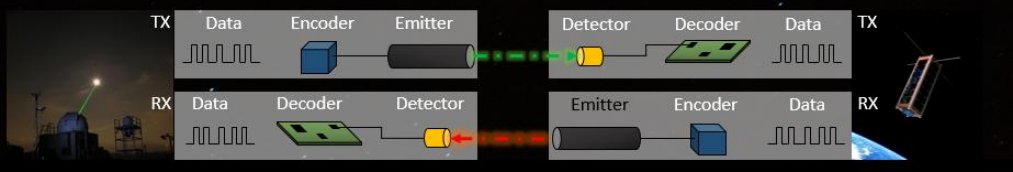
\includegraphics[width=0.8\linewidth]{img/eng_fig_3.png}
 \caption{Two-way CubeSat based optical communications setup. The
 transmitter (TX) and the receiver (RX) \citep{nasa_cube}}
\end{figure}

In helio-synchroneous, one complete orbit taking 90 minutes. Our
satellites orbit the Earth 16 times per day, the cubesat will transmit
data to the ground station. The time window will be 7.5 minutes before
the satellite is below horizon. Within this 7.5 minutes the satellite
and the ground station need to establish a data link and transfer the
data. With optical communication we can transmit 25 MB/s data. The
equation below is used to calculate the required ground based station
number to transfer 1 TB/day for a satellite;

``Unlike radio communications, optical communications are interrupted by
clouds. Therefore, any high availability laser communications system
must include a strategy for ensuring a cloud-free line of sight
(CFLOS)'' \citep{link}.

Even the most cloud-free locations are cloudy about 30$\backslash$% of the time, so
achieving system availabilities higher than 70$\backslash$% requires a mitigation
strategy. The most effective strategy is ``site diversity'', which is
having redundant sites so that if one is clouded out another can be used
as a backup \citep{link}.

To minimize the effect of clouds, number of required ground based
station will be doubled. In addition to this, 1 TB of non-volatile
storage on SD cards will be replaced on satellites.

\subsection{Onboard Instruments}
\label{sec:orgac81367}

One of the main advantages of the Earth observation using nano satellites
technique is a possibility of launching a fleet of satellites with similar
onboard instruments. To achieve global coverage of the Earth surface every 3
hours during \whocares mission a fleet of 90 nanosatellites is needed. Two
spectrometers (for UV-VIS and IR spectral ranges) will be installed on each of
them. Field of view of the instrument is 40° (\textasciitilde{}400x400 km on the surface of the
Earth) with spatial resolution 0.2 km. For clouds 3D structure reconstruction,
it is necessary to observe atmosphere in nadir from two different points on the
orbit. We suggest a scheme of satellites motion when all parts of the fleet move
in pairs with a constant distance between partners – d=200 km. In this case
fields of view of two detectors in pair overlap (\textasciitilde{}200x400 km) and provide
continuous observation of the underlying part of the atmosphere from two orbital
points (Fig. 1). The optical measurement principle is depicted in Fig. 2. The
idea is to use to detector in order to cover the spectral range from 165 nm to
1800 nm. The first detector will be a standard 2048 x 2048 pixels wide CCD or
CMOS in order to cover the UV-VIS spectral range (165 nm - 1100 nm) and a 2048 x
2048 pixels CMOS-like IR-array (surely made from HgCdTe or InGaAs) to cover the
NIR spectral range (800 nm – 1800 nm). The hyperspectrality will be ensured by
using a Fabry-Pérot Fourier transform spectrometry technique to retrieve the
spectral component [1,2]. This will allow to attain the wanted spectral
resolution as well as the hyperspectrality by changing the Fabry-Pérot
resonances and hence sweeping across the bandwidth. Furthermore, the Fabry-Perot
interferometer can be much lighter and more compact than a conventional
interferometer configuration such as Sagnac or Michelson interferometry designs
and hence are suitable for remote sensing applications [2].

\begin{figure}[hbpt]
\centering
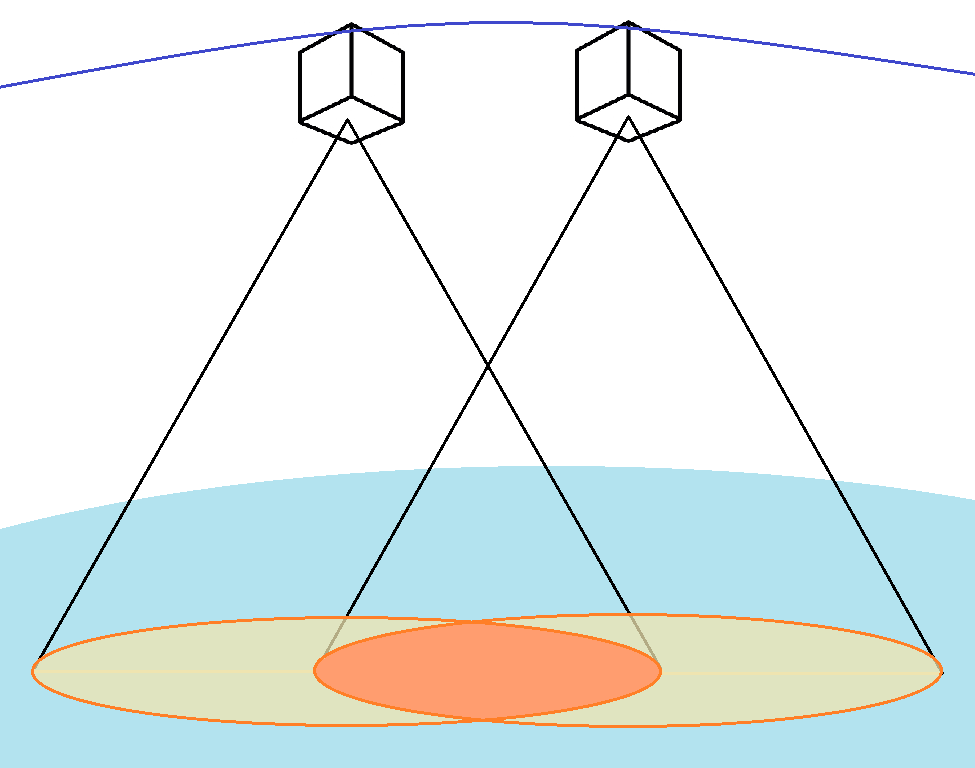
\includegraphics[width=0.6\textwidth]{img/eng_fig_1}
\caption{Overlapping of the field of views of two detectors in pair.}
\end{figure}

\begin{figure}[hbpt]
\centering
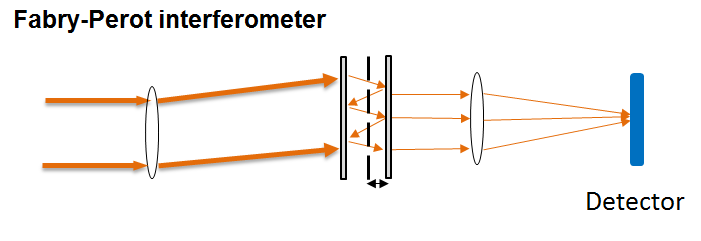
\includegraphics[width=\textwidth]{img/eng_fig_2}
\caption{Overlapping of the field of views of two detectors in pair.}
\end{figure}

\bibliographystyle{apalike}
\bibliography{literature}  
\end{document}
